\documentclass[10pt]{article}
\usepackage[utf8]{inputenc}
\usepackage[T1]{fontenc}
\usepackage{amsmath}
\usepackage{amsfonts}
\usepackage{amssymb}
\usepackage[version=4]{mhchem}
\usepackage{stmaryrd}
\usepackage{graphicx}
\usepackage[export]{adjustbox}
\graphicspath{ {./images/} }
\usepackage{bbold}

\title{14 Quantum mechanics }

\author{}
\date{}


\begin{document}
\maketitle
Our purpose in this chapter is to present the key concepts of quantum mechanics in the language of Hilbert spaces. The reader who has not previously met the physical ideas motivating quantum mechanics, and some of the more elementary applications of Schrödinger's equation, is encouraged to read any of a number of excellent texts on the subject such as $[1-4]$. Otherwise, the statements given here must to a large extent be taken on trust - not an altogether easy thing to do, since the basic assertions of quantum theory are frequently counterintuitive to anyone steeped in the classical view of physics. Quantum mechanics is frequently presented in the form of several postulates, as though it were an axiomatic system such as Euclidean geometry. As often presented, these postulates may not meet the standards of mathematical rigour required for a strictly logical set of axioms, so that little is gained by such an approach. We will do things a little more informally here. For those only interested in the mathematical aspects of quantum mechanics and the role of Hilbert space see [5-8].

Many of the standard applications, such as the hydrogen atom, will be omitted here as they can be found in all standard textbooks, and we leave aside the enormous topic of measurement theory and interpretations of quantum mechanics. This is not to say that we need be totally comfortable with quantum theory as it stands. Undoubtedly, there are some philosophically disquieting features in the theory, often expressed in the form of socalled paradoxes. However, to attempt an 'interpretation' of the theory in order to resolve these apparent paradoxes assumes that there are natural metaphysical concepts. Suitable introductions to this topic can be found in [3, chap. 11] or [4, chap. 5].

\section{14.1 Basic concepts}
\subsection{Photon polarization experiments}
To understand how quantum mechanics works, we look at the outcome of a number of Gedanken experiments involving polarized light beams. Typically, a monochromatic plane wave solution or Maxwell equations (see Problem 9.23) has electric field

$$
\mathbf{E} \propto \operatorname{Re}\left(\alpha \mathbf{e}_{x}+\beta \mathbf{e}_{y}\right) \mathrm{e}^{i(k z-\omega t)}
$$

where $\mathbf{e}_{x}$ and $\mathbf{e}_{y}$ are the unit vectors in the $x$ - and $y$-directions and $\alpha$ and $\beta$ are complex numbers such that

$$
|\alpha|^{2}+|\beta|^{2}=1
$$

When $\alpha / \beta$ is real we have a linearly polarized wave, as for example

$$
\mathbf{E} \propto \frac{1}{\sqrt{2}}\left(\mathbf{e}_{x}+\mathbf{e}_{y}\right) \mathrm{e}^{i(k z-\omega t)}
$$

If $b= \pm i a= \pm i / \sqrt{2}$ the wave is circularly polarized; the + sign is said to be right circularly polarized, and the - sign is left circularly polarized. In all other cases it is said to be elliptically polarized. If we pass a polarized beam through a polarizer with axis of polarization $\mathbf{e}_{x}$, then the beam is reduced in intensity by the factor $|a|^{2}$ and the emergent beam is $\mathbf{e}_{x}$-polarized. Thus, if the resultant beam is passed through another $\mathbf{e}_{x}$-polarizer it will be $100 \%$ transmitted, while if it is passed through an $\mathbf{e}_{y}$-polarizer it will be totally absorbed and nothing will come through. This is the classical situation.

As was discovered by Planck and Einstein at the turn of the twentieth century, light beams come in discrete packets called photons, having energy $E=h v=\hbar \omega$ where $h \approx$ $6.625 \times 10^{-27} \mathrm{~g} \mathrm{~cm}^{2} \mathrm{~s}^{-1}$ is Planck's constant and $\hbar=h / 2 \pi$. What happens if we send the beams through the polarizers one photon at a time? Since the frequency of each photon is unchanged it emerges with the same energy, and since the intensity of the beam is related to the energy, it must mean that the number of photons is reduced. However, the most obvious conclusion that the beam consists of a mixture of photons consisting of a fraction $|\alpha|^{2}$ polarized in the $\mathbf{e}_{x}$-direction and $|\beta|^{2}$ in the $\mathbf{e}_{y}$-direction will not stand up to scrutiny. For, if a beam with $\alpha=\beta=1 / \sqrt{2}$ were passed through a polarizer designed to only transmit waves linearly polarized in the $\left(\mathbf{e}_{x}+\mathbf{e}_{y}\right) / \sqrt{2}$ direction, then it should be $100 \%$ transmitted. However, on the mixture hypothesis only half the $\mathbf{e}_{x}$-polarized photons should get through, and half the $\mathbf{e}_{y}$-polarized photons, leaving a total fraction $\frac{1}{2} \cdot \frac{1}{2}+\frac{1}{2} \cdot \frac{1}{2}=\frac{1}{2}$ being transmitted.

In quantum mechanics it is proposed that each photon is a 'complex superposition' $\alpha \mathbf{e}_{x}+\beta \mathbf{e}_{y}$ of the two polarization states $\mathbf{e}_{x}$ and $\mathbf{e}_{y}$. The probability of transmission by an $\mathbf{e}_{x}$-polarizer is given by $|\alpha|^{2}$, while the probability of transmission by an $\mathbf{e}_{y}$-polarizer is $|\beta|^{2}$. The effect of the $\mathbf{e}_{x}$-polarizer is essentially to 'collapse' the photon into an $\mathbf{e}_{x}$-polarized state. The polarizer can be regarded both as a measuring device or equally as a device for preparing photons in an $\mathbf{e}_{x}$-polarized state. If used as a measuring device it returns the value 1 if the photon is transmitted, or 0 if not - in either case the act of measurement has changed the state of the photon being measured.

An interesting arrangement to illustrate the second point of view is shown in Fig. 14.1. Consider a beam of photons incident on an $\mathbf{e}_{x}$-polarizer, followed by an $\mathbf{e}_{y}$-polarizer; the net result is that no photons come out of the second polarizer. Now introduce a polarizer for the direction $(1 / \sqrt{2})\left(\mathbf{e}_{x}+\mathbf{e}_{y}\right)$ - in other words a device that should block some of the photons between the two initial polarizers. If the mixture theory were correct, it is inconceivable that this could increase transmission. Yet the reality is that half the photons emerge from this intermediary polarizer with polarization $(1 / \sqrt{2})\left(\mathbf{e}_{x}+\mathbf{e}_{y}\right)$, and a further half of these, namely a quarter in all, are now transmitted by the $\mathbf{e}_{y}$-polarizer.

How can we find the transmission probability of a polarized state $\mathbf{A}$ with respect to an arbitrary polarization direction $\mathbf{B}$ ? The following argument is designed to be motivational rather than rigorous. Let $\mathbf{A}=\alpha \mathbf{e}_{x}+\beta \mathbf{e}_{y}$, where $\alpha$ and $\beta$ are complex numbers subject to $|\alpha|^{2}+|\beta|^{2}=1$. We write $\alpha=\left\langle\mathbf{e}_{x} \mid \mathbf{A}\right\rangle$, called the amplitude for $\mathbf{e}_{x}$-transmission of an
(a)

\begin{center}
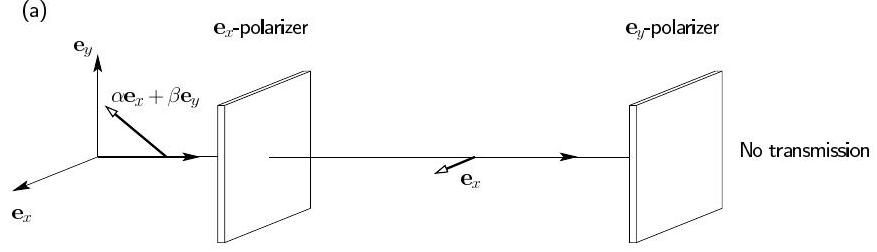
\includegraphics[max width=\textwidth]{2023_12_20_5d48e1c38160b1e32b28g-03}
\end{center}

(b) $\quad \frac{1}{\sqrt{2}}\left(\mathbf{e}_{x}+\mathbf{e}_{y}\right)$-polarizer

\begin{center}
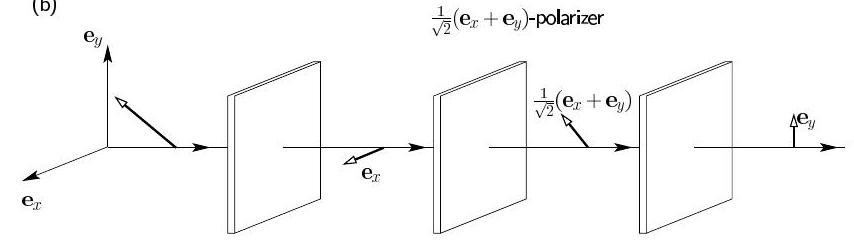
\includegraphics[max width=\textwidth]{2023_12_20_5d48e1c38160b1e32b28g-03(1)}
\end{center}

Figure 14.1 Photon polarization experiment

A-polarized photon. It is a complex number having no obvious physical interpretation of itself, but its magnitude square $|\alpha|^{2}$ is the probability of transmission by an $\mathbf{e}_{x}$-polarizer. Similarly $\beta=\left\langle\mathbf{e}_{y} \mid \mathbf{A}\right\rangle$ is the amplitude for $\mathbf{e}_{y}$-transmission, and $|\beta|^{2}$ the probability of transmission by an $\mathbf{e}_{y}$-polarizer. What is the polarization $A^{\perp}$ such that a polarizer of this type allows for no transmission, $\left\langle\mathbf{A}^{\perp} \mid \mathbf{A}\right\rangle=0$ ? For linearly polarized waves with $\alpha$ and $\beta$ both real we expect it to be geometrically orthogonal, $\mathbf{A}^{\perp}=\beta \mathbf{e}_{x}-\alpha \mathbf{e}_{y}$. For circularly polarized waves, the orthogonal 'direction' is the opposite circular sense. Hence

$$
\frac{1}{\sqrt{2}}\left(\mathbf{e}_{x} \pm i \mathbf{e}_{y}\right)^{\perp}=\frac{1}{\sqrt{2}}\left(\mathbf{e}_{x} \mp i \mathbf{e}_{y}\right) \equiv \mp \frac{1}{\sqrt{2}}\left(i \mathbf{e}_{x}-\mathbf{e}_{y}\right)
$$

since phase factors such as $\pm i$ are irrelevant. In the general elliptical case we might guess that $\mathbf{A}^{\perp}=\bar{\beta} \mathbf{e}_{x}-\bar{\alpha} \mathbf{e}_{y}$, since it reduces to the correct answer for linear and circular polarization. Solving for $\mathbf{e}_{x}$ and $\mathbf{e}_{y}$ we have

$$
\mathbf{e}_{x}=\bar{\alpha} \mathbf{A}+\beta \mathbf{A}^{\perp}, \quad \mathbf{e}_{y}=\bar{\beta} \mathbf{A}-\alpha \mathbf{A}^{\perp}
$$

Let $\mathbf{B}=\gamma \mathbf{e}_{x}+\delta \mathbf{e}_{y}$ be any other polarization, then substituting for $\mathbf{e}_{x}$ and $\mathbf{e}_{y}$ gives

$$
\mathbf{B}=(\gamma \bar{\alpha}+\delta \bar{\beta}) \mathbf{A}+(\gamma \beta-\alpha \delta) \mathbf{A}^{\perp}
$$

Setting $\mathbf{B}=\mathbf{A}$ gives the normalization condition $|\alpha|^{2}+|\beta|^{2}=1$. Hence, since $\langle\mathbf{A} \mid \mathbf{A}\rangle=1$ (transmission probability of 1),

$$
\langle\mathbf{B} \mid \mathbf{A}\rangle=(\gamma \bar{\alpha}+\delta \bar{\beta})=\overline{\langle\mathbf{A} \mid \mathbf{B}\rangle}
$$

Other systems such as the Stern-Gerlach experiment, in which an electron of magnetic moment $\boldsymbol{\mu}$ is always deflected in a magnetic field $\mathbf{H}$ in just two directions, exhibit a completely analogous formalism. The conclusion is that the quantum mechanical states of a system form a complex vector space with inner product $\langle\phi \mid \psi\rangle$ satisfying the usual conditions

$$
\left\langle\phi \mid \alpha \psi_{1}+\beta \psi_{2}\right\rangle=\alpha\left\langle\phi \mid \psi_{1}\right\rangle+\beta\left\langle\phi \mid \psi_{2}\right\rangle \quad \text { and } \quad\langle\phi \mid \psi\rangle=\overline{\langle\psi \mid \phi\rangle} \text {. }
$$

The probability of obtaining a value corresponding to $\phi$ in a measurement is

$$
P(\phi, \psi)=|\langle\phi \mid \psi\rangle|^{2}
$$

As will be seen, states are in fact normalized to $\langle\psi \mid \psi\rangle=1$, so that only linear combinations $\alpha \psi_{1}+\beta \psi_{2}$ with $|\alpha|^{2}+|\beta|^{2}=1$ are permitted.

\subsection{The Hilbert space of states}
We will now assume that every physical system corresponds to a separable Hilbert space $\mathcal{H}$, representing all possible states of the system. The Hilbert space may be finite dimensional, as for example the states of polarization of a photon or electron, but often it is infinite dimensional. A state of the system is represented by a non-zero vector $\psi \in \mathcal{H}$, but this correspondence is not one-to-one, as any two vectors $\psi$ and $\psi^{\prime}$ that are proportional through a non-zero complex factor, $\psi^{\prime}=\lambda \psi$ where $\lambda \in \mathbb{C}$, will be assumed to represent identical states. In other words, a state is an equivalence class or ray of vectors [ $\psi]$ all related by proportionality. A state may be represented by any vector from the class, and it is standard to select a representative having unit norm $\|\psi\|=1$. Even this restriction does not uniquely define a vector to represent the state, as any other vector $\psi^{\prime}=\lambda \psi$ with $|\lambda|=1$ will also satisfy the unit norm condition. The angular freedom, $\lambda=\mathrm{e}^{i c}$, is sometimes referred to as the phase of the state vector. Phase is only significant in a relative sense; for example, $\psi+\mathrm{e}^{i c} \phi$ is in general a different state to $\psi+\phi$, but $\mathrm{e}^{i c}(\psi+\phi)$ is not.

In this chapter we will adopt Dirac's bra-ket notation which, though slightly quirky, has largely become the convention of choice among physicists. Vectors $\psi \in \mathcal{H}$ are written as kets $|\psi\rangle$ and one makes the identification $|\lambda \psi\rangle=\lambda|\psi\rangle$. By the Riesz representation theorem 13.10, to each linear functional $f: \mathcal{H} \rightarrow \mathbb{C}$ there corresponds a unique vector $\phi \equiv$ $|\phi\rangle \in \mathcal{H}$ such that $f(\psi)=\langle\phi \mid \psi\rangle$. In Dirac's terminology the linear functional is referred to as a bra, written $\langle\phi|$. The relation between bras and kets is antilinear,

$$
\langle\lambda \psi+\phi|=\bar{\lambda}\langle\psi|+\langle\phi| .
$$

In Dirac's notation it is common to think of a linear operator $\left(A, D_{A}\right)$ as acting to the left on kets (vectors), while acting to the right on bras (linear functionals):

$$
A|\psi\rangle \equiv|A \psi\rangle
$$

and if $\phi \in D_{A^{*}}$

$$
\langle\phi| A \equiv\left\langle A^{*} \phi\right| .
$$

The following notational usages for the matrix elements of an operator between two vectors are all equivalent:

$$
\langle\phi|A| \psi\rangle \equiv\langle\phi \mid A \psi\rangle=\left\langle A^{*} \phi \mid \psi\right\rangle=\overline{\left\langle\psi \mid A^{*} \phi\right\rangle}=\overline{\left\langle\psi\left|A^{*}\right| \phi\right\rangle} .
$$

If $\left|e_{i}\right\rangle$ is an o.n. basis of kets in a separable Hilbert space then we may write

$$
A\left|e_{j}\right\rangle=\sum_{i} a_{i j}\left|e_{i}\right\rangle \quad \text { where } \quad a_{i j}=\left\langle e_{i}|A| e_{j}\right\rangle
$$

\subsection{Observables}
In classical mechanics, physical observables refer to quantities such as position, momentum, energy or angular momentum, which are real numbers or real multicomponented objects. In quantum mechanics observables are represented by self-adjoint operators on the Hilbert space of states. We first consider the case where $A$ is a hermitian operator (bounded and continuous). Such an observable is said to be complete if the corresponding hermitian operator $A$ is complete, so that there is an orthonormal basis made up of eigenvectors $\left|\psi_{1}\right\rangle,\left|\psi_{2}\right\rangle, \ldots$ such that

$$
A\left|\psi_{n}\right\rangle=\alpha_{n}\left|\psi_{n}\right\rangle \quad \text { where } \quad\left\langle\psi_{m} \mid \psi_{n}\right\rangle=\delta_{m n}
$$

The result of measuring a complete observable is always one of the eigenvalues $\alpha_{n}$, and the fact that these are real numbers provides a connection with classical physics. By Theorem 13.2 every state $|\psi\rangle$ can be written uniquely in the form

$$
|\psi\rangle=\sum_{n=1}^{\infty} c_{n}\left|\psi_{n}\right\rangle \quad \text { where } \quad c_{n}=\left\langle\psi_{n} \mid \psi\right\rangle
$$

or, since the vector $|\psi\rangle$ is arbitrary, we can write

$$
I \equiv \mathrm{id}_{\mathcal{H}}=\sum_{n=1}^{\infty}\left|\psi_{n}\right\rangle\left\langle\psi_{n}\right|
$$

Exercise: Show that the operator $A$ can be written in the form

$$
A=\sum_{n=1}^{\infty} \alpha_{n}\left|\psi_{n}\right\rangle\left\langle\psi_{n}\right|
$$

The matrix element of the identity operator between two states $|\phi\rangle$ and $|\psi\rangle$ is

$$
\langle\phi \mid \psi\rangle=\langle\phi|I| \psi\rangle=\sum_{n=1}^{\infty}\left\langle\phi \mid \psi_{n}\right\rangle\left\langle\psi_{n} \mid \psi\right\rangle
$$

Its physical interpretation is that $|\langle\phi \mid \psi\rangle|^{2}$ is the probability of realizing a state $|\psi\rangle$ when the system is in the state $|\phi\rangle$. Since both state vectors are unit vectors, the Cauchy-Schwarz inequality ensures that the probability is less than one,

$$
|\langle\phi \mid \psi\rangle|^{2} \leq\|\phi\|^{2}\|\psi\|^{2}=1
$$

If $A$ is a complete hermitian operator with eigenstates $\left|\psi_{n}\right\rangle$ satisfying Eq. (14.1) then, according to this assumption, the probability that the eigenstate $\left|\psi_{n}\right\rangle$ is realized when the system is in the state $|\psi\rangle$ is given by $\left|c_{n}\right|^{2}=\left|\left\langle\psi_{n} \mid \psi\right\rangle\right|^{2}$ where the $c_{n}$ are the coefficients in the expansion (14.2). Thus $\left|c_{n}\right|^{2}$ is the probability that the value $\alpha_{n}$ be obtained on measuring
the observable $A$ when the system is in the state $|\psi\rangle$. By Parseval's identity (13.7) we have

$$
\sum_{n=1}^{\infty}\left|c_{n}\right|^{2}=\|\psi\|^{2}=1
$$

and the expectation value of the observable $A$ in a given state $|\psi\rangle$ is given by

$$
\langle A\rangle \equiv\langle A\rangle_{\psi}=\sum_{n=1}^{\infty}\left|c_{n}\right|^{2} \alpha_{n}=\langle\psi|A| \psi\rangle
$$

The act of measuring the observable $A$ 'collapses' the system into one of the eigenstates $\left|\psi_{n}\right\rangle$, with probability $\left|c_{n}\right|^{2}=\left|\left\langle\psi_{n} \mid \psi\right\rangle\right|^{2}$. This feature of quantum mechanics, that the result of a measurement can only be known to within a probability, and that the system is no longer in the same state after a measurement as before, is one of the key differences between quantum and classical physics, where a measurement is always made delicately enough so as to minimally disturb the system. Quantum mechanics asserts that this is impossible, even in principle.

The root mean square deviation $\Delta A$ of an observable $A$ in a state $|\psi\rangle$ is defined by

$$
\Delta A=\sqrt{\left\langle(A-\langle A\rangle I)^{2}\right\rangle}
$$

The quantity under the square root is positive, for

$$
\left\langle(A-\langle A\rangle I)^{2}\right\rangle=\left\langle\psi \mid(A-\langle A\rangle I)^{2} \psi\right\rangle=\|(A-\langle A\rangle I) \psi\|^{2} \geq 0
$$

since $A$ is hermitian and $\langle A\rangle$ is real. A useful formula for the RMS deviation is

$$
\begin{aligned}
(\Delta A)^{2} & =\left\langle\psi\left|A^{2}-2 A\langle A\rangle+\langle A\rangle^{2} I\right| \psi\right\rangle \\
& =\left\langle A^{2}\right\rangle-\langle A\rangle^{2}
\end{aligned}
$$

Hence $|\psi\rangle$ is an eigenstate of $A$ if and only if it is dispersion-free, $\Delta A=0$. For, by (14.5), if $A|\psi\rangle=\alpha|\psi\rangle$ then $\langle A\rangle=\alpha$ and $\left\langle A^{2}\right\rangle=\alpha^{2}$ immediately results in $\Delta A=0$, and conversely if $\Delta A=0$ then $\|(A-\langle A\rangle I) \psi\|^{2}$, which is only possible if $A|\psi\rangle=\langle A\rangle|\psi\rangle$. Dispersion-free states are sometimes referred to as pure states with respect to the observable $A$.

Theorem 14.1 (Heisenberg) Let $A$ and $B$ be two hermitian operators, then for any state $|\psi\rangle$

$$
\Delta A \Delta B \geq \frac{1}{2}|\langle[A, B]\rangle|
$$

where $[A, B]=A B-B A$ is the commutator of the two operators.

Proof: Let

$$
\left|\psi_{1}\right\rangle=(A-\langle A\rangle I)|\psi\rangle, \quad\left|\psi_{2}\right\rangle=(B-\langle B\rangle I)|\psi\rangle
$$

so that $\Delta A=\left\|\psi_{1}\right\|$ and $\Delta B=\left\|\psi_{2}\right\|$. Using the Cauchy-Schwarz inequality,

$$
\begin{aligned}
\Delta A \Delta B=\left\|\psi_{1}\right\|\left\|\psi_{2}\right\| & \geq\left|\left\langle\psi_{1} \mid \psi_{2}\right\rangle\right| \\
& \geq\left|\operatorname{Im}\left\langle\psi_{1} \mid \psi_{2}\right\rangle\right| \\
& =\left|\frac{1}{2 i}\left(\left\langle\psi_{1} \mid \psi_{2}\right\rangle-\left\langle\psi_{2} \mid \psi_{1}\right\rangle\right)\right| .
\end{aligned}
$$

Now

$$
\begin{aligned}
\left\langle\psi_{1} \mid \psi_{2}\right\rangle & =\langle(A-\langle A\rangle I) \psi \mid(B-\langle B\rangle I) \psi\rangle \\
& =\langle\psi|A B| \psi\rangle-\langle A\rangle\langle B\rangle .
\end{aligned}
$$

Hence

$$
\Delta A \Delta B \geq \frac{1}{2}|\langle\psi|A B-B A| \psi\rangle|=\frac{1}{2}|\langle[A, B]\rangle| .
$$

Exercise: Show that for any two hermitian operators $A$ and $B$, the operator $i[A, B]$ is hermitian.

Exercise: Show that $\langle[A, B]\rangle=0$ for any state $|\psi\rangle$ that is an eigenvector of either $A$ or $B$.

A particularly interesting case of Theorem 14.1 occurs when $A$ and $B$ satisfy the canonical commutation relations,

$$
[A, B]=i \hbar I
$$

where $\hbar=h / 2 \pi$ is Planck's constant divided by $2 \pi$. Such a pair of observables are said to be complementary. With some restriction on admissible domains they hold for the position operator $Q=A_{x}$ and the momentum operator $P=-i \hbar \mathrm{d} / \mathrm{d} x$ discussed in Examples 13.19 and 13.20. For, let $f$ be a function in the intersection of their domains, then

$$
[Q, P]=x\left(-i \hbar \frac{\mathrm{d} f}{\mathrm{~d} x}\right)+i \hbar \frac{\mathrm{d}(x f)}{\mathrm{d} x}=i \hbar f
$$

whence

$$
[Q, P]=i \hbar I
$$

Theorem 14.1 results in the classic Heisenberg uncertainty relation

$$
\Delta Q \Delta P \geq \frac{\hbar}{2}
$$

Sometimes it is claimed that this relation has no effect at a macroscopic level because Planck's constant $h$ is so 'small' ( $h \approx 6.625 \times 10^{-27} \mathrm{~g} \mathrm{~cm}^{2} \mathrm{~s}^{-1}$ ). Little could be further from the truth. The fact that we are supported by a solid Earth, and not collapse in towards its centre, can be traced to this and similar relations.

Exercise: Show that Eq. (14.7) cannot possibly hold in a finite dimensional space. [Hint: Take the trace of both sides.]

Theorem 14.2 A pair of complete hermitian observables $A$ and $B$ commute, $[A, B]=0$, if and only if there exists a complete set of common eigenvectors. Such observables are said to be compatible.

Proof: If there exists a basis of common eigenvectors $\left|\psi_{1}\right\rangle,\left|\psi_{2}\right\rangle, \ldots$ such that

$$
A\left|\psi_{n}\right\rangle=\alpha_{n}\left|\psi_{n}\right\rangle, \quad B\left|\psi_{n}\right\rangle=\beta_{n}\left|\psi_{n}\right\rangle,
$$

then $A B\left|\psi_{n}\right\rangle=\alpha_{n} \beta_{n}\left|\psi_{n}\right\rangle=B A\left|\psi_{n}\right\rangle$ for each $n$. Hence for arbitrary vectors $\psi$ we have from (14.2)

$$
[A, B]|\psi\rangle=(A B-B A) \sum_{n}\left|\psi_{n}\right\rangle\left\langle\psi_{n} \mid \psi\right\rangle=0
$$

Conversely, suppose that $A$ and $B$ commute. Let $\alpha$ be an eigenvalue of $A$ with eigenspace $\left.M_{\alpha}=\{|\psi\rangle|A| \psi\rangle=\alpha|\psi\rangle\right\}$, and set $P_{\alpha}$ to be the projection operator into this subspace. If $|\psi\rangle \in M_{\alpha}$ then $B|\psi\rangle \in M_{\alpha}$, since

$$
A B|\psi\rangle=B A|\psi\rangle=B \alpha|\psi\rangle=\alpha B|\psi\rangle
$$

For any $|\phi\rangle \in \mathcal{H}$ we therefore have $B P_{\alpha}|\phi\rangle \in M_{\alpha}$. Hence

$$
P_{\alpha} B P_{\alpha}|\phi\rangle=B P_{\alpha}|\phi\rangle
$$

and since $|\phi\rangle$ is an arbitrary vector,

$$
P_{\alpha} B P_{\alpha}=B P_{\alpha}
$$

Taking the adjoint of this equation, and using $B^{*}=B, P_{\alpha}=P_{\alpha}^{*}$, gives

$$
P_{\alpha} B P_{\alpha}=P_{\alpha}^{*} B^{*} P_{\alpha}^{*}=P_{\alpha}^{*} B^{*}=P_{\alpha} B
$$

and it follows that $P_{\alpha} B=B P_{\alpha}$, the operator $B$ commutes with all projection operators $P_{\alpha}$.

If $\beta$ is any eigenvalue of $B$ with projection map $P_{\beta}$, then since $P_{\alpha}$ is a hermitian operator that commutes with $B$ the above argument shows that it commutes with $P_{\beta}$,

$$
P_{\alpha} P_{\beta}=P_{\beta} P_{\alpha}
$$

Hence, the operator $P_{\alpha \beta}=P_{\alpha} P_{\beta}$ is hermitian and idempotent, and using Theorem 13.14 it is a projection operator. The space it projects into is $M_{\alpha \beta}=M_{\alpha} \cap M_{\beta}$. Two such spaces $M_{\alpha \beta}$ and $M_{\alpha^{\prime} \beta^{\prime}}$ are clearly orthogonal unless $\alpha=\alpha^{\prime}$ and $\beta=\beta^{\prime}$. Choose an orthonormal basis for each $M_{\alpha \beta}$. The collection of these vectors is a complete o.n. set consisting entirely of common eigenvectors to $A$ and $B$. For, if $|\phi\rangle \neq 0$ is any non-zero vector orthogonal to all $M_{\alpha \beta}$, then $P_{\alpha} P_{\beta}|\phi\rangle \neq 0$ for all $\alpha, \beta$. Since $A$ is complete this implies $P_{\beta}|\phi\rangle=0$ for all eigenvalues $\beta$ of $B$, and since $B$ is complete we must have $|\phi\rangle=0$.

Example 14.1 Consider spin $\frac{1}{2}$ electrons in a Stern-Gerlach device for measuring spin in the $z$-direction. Let $\sigma_{z}$ be the operator for the observable 'spin in the $z$-direction'. It can only take on two values - up or down. This results in two eigenvalues \textbackslash pm 1 , and the eigenvectors are written

$$
\sigma_{z}|+z\rangle=|+z\rangle, \quad \sigma_{z}|-z\rangle=-|-z\rangle
$$

Thus

$$
\sigma_{z}=|+z\rangle\langle+z|-|-z\rangle\langle-z|, \quad I=|+z\rangle\langle+z|+|-z\rangle\langle-z|
$$

and setting $\left|e_{1}\right\rangle=|+z\rangle,\left|e_{2}\right\rangle=|-z\rangle$ results in the matrix components

$$
\left(\sigma_{z}\right)_{i j}=\left\langle e_{1}\left|\sigma_{z}\right| e_{j}\right\rangle=\left(\begin{array}{cc}
1 & 0 \\
0 & -1
\end{array}\right)
$$

Every state of the system can be written

$$
|\psi\rangle=\psi_{1}|+z\rangle+\psi_{2}|-z\rangle \quad \text { where } \quad \psi_{i}=\left\langle e_{i} \mid \psi\right\rangle
$$

The operator $\sigma_{\mathbf{n}}$ representing spin in an arbitrary direction

$$
\mathbf{n}=\cos \theta \mathbf{e}_{z}+\sin \theta \cos \phi \mathbf{e}_{x}+\sin \theta \sin \phi \mathbf{e}_{y}
$$

has expectation values in different directions given by the classical values

$$
\begin{aligned}
\left\langle+z\left|\sigma_{\mathbf{n}}\right|+z\right\rangle & =\cos \theta \\
\left\langle+x\left|\sigma_{\mathbf{n}}\right|+x\right\rangle & =\sin \theta \cos \phi \\
\left\langle+y\left|\sigma_{\mathbf{n}}\right|+y\right\rangle & =\sin \theta \sin \phi
\end{aligned}
$$

where $| \pm x\rangle$ refers to the pure states in the $x$ direction, $\sigma_{x}| \pm x\rangle= \pm| \pm x\rangle$, etc.

Since $\sigma_{\mathbf{n}}$ is hermitian with eigenvalues $\lambda_{i}= \pm 1$ its matrix with respect to any o.n. basis has the form

$$
\left(\sigma_{\mathbf{n}}\right)_{i j}=\left(\begin{array}{ll}
\alpha & \beta \\
\beta & \delta
\end{array}\right)
$$

where

$$
\alpha+\delta=\lambda_{1}+\lambda_{2}=0, \quad \alpha \delta-\beta \bar{\beta}=\lambda_{1} \lambda_{2}=-1
$$

Hence $\delta=-\alpha$ and $\alpha^{2}=1-|\beta|^{2}$. The expectation value of $\sigma_{\mathbf{n}}$ in the $|+z\rangle$ state is given by

$$
\left\langle+z\left|\sigma_{\mathbf{n}}\right|+z\right\rangle=\left(\sigma_{\mathbf{n}}\right)_{11}=\alpha=\cos \theta
$$

so that $\beta=\sin \theta \mathrm{e}^{-i c}$ where $c$ is a real number. For $\mathbf{n}=\mathbf{e}_{x}$ and $\mathbf{n}=\mathbf{e}_{y}$ we have $\cos \theta=0$,

$$
\sigma_{x}=\left(\begin{array}{cc}
0 & \mathrm{e}^{-i a} \\
\mathrm{e}^{i a} & 0
\end{array}\right), \quad \sigma_{y}=\left(\begin{array}{cc}
0 & \mathrm{e}^{-i b} \\
\mathrm{e}^{i b} & 0
\end{array}\right)
$$

The states $| \pm x\rangle$ and $| \pm y\rangle$ are the eigenstates of $\sigma_{x}$ and $\sigma_{y}$ with normalized components

$$
| \pm x\rangle=\frac{1}{\sqrt{2}}\left(\begin{array}{c}
\mathrm{e}^{-i a} \\
\pm 1
\end{array}\right), \quad| \pm y\rangle=\frac{1}{\sqrt{2}}\left(\begin{array}{c}
\mathrm{e}^{-i b} \\
\pm 1
\end{array}\right)
$$

and as the expection values of $\sigma_{x}$ in the orthogonal states $| \pm y\rangle$ vanish,

$$
\left\langle+y\left|\sigma_{x}\right|+y\right\rangle=\frac{1}{2}\left(\mathrm{e}^{i(b-a)}+\mathrm{e}^{i(a-b)}\right)=\cos (b-a)=0 .
$$

Hence $b=a+\pi / 2$. Applying the unitary operator $U$

$$
U=\left(\begin{array}{cc}
\mathrm{e}^{i a} & 0 \\
0 & 1
\end{array}\right)
$$

results in $a=0$, and the spin operators are given by the Pauli representation

$$
\sigma_{x}=\sigma_{1}=\left(\begin{array}{cc}
0 & 1 \\
1 & 0
\end{array}\right), \quad \sigma_{y}=\sigma_{2}=\left(\begin{array}{cc}
0 & -i \\
i & 0
\end{array}\right), \quad \sigma_{z}=\sigma_{3}=\left(\begin{array}{cc}
1 & 0 \\
0 & -1
\end{array}\right)
$$

For a spin operator in an arbitrary direction the expectation values are $\left\langle+x\left|\sigma_{\mathbf{n}}\right|+x\right\rangle=$ $\sin \theta \cos \phi$, etc., from which it is straightforward to verify that

$$
\sigma_{\mathbf{n}}=\left(\begin{array}{cc}
\cos \theta & \sin \theta \mathrm{e}^{-i \phi} \\
\sin \theta \mathrm{e}^{i \phi} & -\cos \theta
\end{array}\right)=\sin \theta \cos \phi \sigma_{x}+\sin \theta \sin \phi \sigma_{y}+\cos \theta \sigma_{z}
$$

Exercise: Find the eigenstates $|+\mathbf{n}\rangle$ and $|-\mathbf{n}\rangle$ of $\sigma_{\mathbf{n}}$.

\subsection{Unbounded operators in quantum mechanics}
An important part of the framework of quantum mechanics is the correspondence principle, which asserts that to every classical dynamical variable there corresponds a quantum mechanical observable. This is at best a sort of guide - for example, as there is no natural way of defining general functions $f(Q, P)$ for a pair of non-commuting operators such as $Q$ and $P$, it is not clear what operators correspond to generalized position and momentum in classical canonical coordinates. For rectangular cartesian coordinates $x, y, z$ and momenta $p_{x}=m \dot{x}$, etc. experience has taught that the Hilbert space of states corresponding to a one-dimensional dynamical system is $\mathcal{H}=L^{2}(\mathbb{R})$, and the position and momentum operators are given by

$$
Q \psi(x)=x \psi(x) \text { and } P \psi(x)=-i \hbar \frac{\mathrm{d} \psi}{\mathrm{d} x}
$$

These operators are unbounded operators and have been discussed in Examples 13.17, 13.19 and 13.20 of Chapter 13 .

As these operators are not defined on all of $\mathcal{H}$ it is most common to take domains

$$
\begin{aligned}
& D_{Q}=\left\{\left.\psi(x) \in L^{2}(\mathbb{R})\left|\int_{-\infty}^{\infty} x^{2}\right| \psi(x)\right|^{2} \mathrm{~d} x<\infty\right\}, \\
& D_{P}=\left\{\psi(x) \in L^{2}(\mathbb{R}) \mid \psi(x) \text { is differentiable and } \int_{-\infty}^{\infty}\left\|\frac{\mathrm{d} \psi(x)}{\mathrm{d} x}\right\|^{2} \mathrm{~d} x<\infty\right\} .
\end{aligned}
$$

These domains are dense in $L^{2}(\mathbb{R})$ since the basis of functions $\phi_{n}(x)$ constructed from hermite polynomials in Example 13.7 (see Eq. (13.6)) belong to both of them. As shown in Example 13.19 the operator $\left(Q, D_{Q}\right)$ is self-adjoint, but $\left(P, D_{P}\right)$ is a symmetric operator that is not self-adjoint (see Example 13.20). To make it self-adjoint it must be extended to the domain of absolutely continuous functions.

Example 14.2 The position operator $Q$ has no eigenvalues and eigenfunctions in $L^{2}(\mathbb{R})$ (see Example 13.14). For the momentum operator $P$ the eigenvalue equation reads

$$
\frac{\mathrm{d} \psi}{\mathrm{d} x}=i \lambda \psi(x) \Longrightarrow \psi(x)=\mathrm{e}^{i \lambda x}
$$

and even when $\lambda$ is a real number the function $\psi(x)$ does not belong to $D_{P}$,

$$
\int_{-\infty}^{\infty}\left|\mathrm{e}^{i \lambda x}\right|^{2} \mathrm{~d} x=\int_{-\infty}^{\infty} 1 \mathrm{~d} x=\infty
$$

For each real number $k$ set $\varepsilon_{k}(x)=\mathrm{e}^{i k x}$, and

$$
\left\langle\varepsilon_{k} \mid \psi\right\rangle=\int_{-\infty}^{\infty} \mathrm{e}^{-i k x} \psi(x) \mathrm{d} x
$$

is a linear functional on $L^{2}(\mathbb{R})$ - in fact, it is the Fourier transform of Section 12.3. This linear functional can be thought of as a tempered distribution $\left\langle\varepsilon_{k}\right|$ on the space of test functions of rapid decrease $D_{P}$. It is a bra that corresponds to no ket vector $\left|\varepsilon_{k}\right\rangle$ (this does not violate the Riesz representation theorem 13.10 since the domain $D_{P}$ is not a closed subspace of $L^{2}(\mathbb{R})$ ). In quantum theory it is common to write equations that may be interpreted as

$$
\left\langle\varepsilon_{k}\right| P=k\left\langle\varepsilon_{k}\right|
$$

which hold in the distributional sense,

$$
\left\langle\varepsilon_{k}|P| \psi\right\rangle=k\left\langle\varepsilon_{k} \mid \psi\right\rangle \quad \text { for all } \psi \in D_{P}
$$

Its integral version holds if we permit integration by parts, as for distributions,

$$
\int_{-\infty}^{\infty} \mathrm{e}^{-i k x}\left(-i \frac{\mathrm{d} \psi(x)}{\mathrm{d} x}\right) \mathrm{d} x=\int_{-\infty}^{\infty} i \frac{\mathrm{de}^{-i k x}}{\mathrm{~d} x} \psi(x) \mathrm{d} x=k \int_{-\infty}^{\infty} \mathrm{e}^{-i k x} \psi(x) \mathrm{d} x
$$

Similarly, for each real $a$ define the linear functional $\left\langle\delta_{a}\right|$ by

$$
\left\langle\delta_{a} \mid \psi\right\rangle=\psi(a)
$$

for all kets $|\psi\rangle \equiv \psi(x) \in D_{Q}$. These too can be thought of as distributions on a set of test functions of rapid decrease. They behave as 'eigenbras' of the position operator $Q$,

$$
\left\langle\delta_{a}\right| Q=a\left\langle\delta_{a}\right|
$$

since

$$
\begin{aligned}
\left\langle\delta_{a}|Q| \psi\right\rangle & =\left\langle\delta_{a} \mid x \psi(x)\right\rangle \\
& =a \psi(a)=a\left\langle\delta_{a} \mid \psi\right\rangle
\end{aligned}
$$

for all $|\psi\rangle \in D_{Q}$. While there is no function $\delta_{a}(x)$ in $L^{2}(\mathbb{R})$ having $\left\langle\delta_{a}\right|$, the Dirac delta function $\delta_{a}(x)=\delta(x-a)$ can be thought of as fulfilling this role in a distributional sense (see Chapter 12).

For a self-adjoint operator $A$ we may apply Theorem 13.25. Let $E_{\lambda}$ be the spectral family of increasing projection operators defined by $A$, such that

$$
A=\int_{-\infty}^{\infty} \lambda \mathrm{d} E_{\lambda} \quad \text { and } \quad I=\int_{-\infty}^{\infty} \mathrm{d} E_{\lambda}
$$

The latter relation follows from

$$
1=\langle\psi \mid \psi\rangle=\int_{-\infty}^{\infty} \mathrm{d}\left\langle\psi \mid E_{\lambda} \psi\right\rangle
$$

for all $\psi \in D_{A}$.

Exercise: Prove Eq. (14.12).

If $S$ is any measurable subset of $\mathbb{R}$ then the probability of the measured value of $A$ lying in $S$, when the system is in a state $|\psi\rangle$, is given by

$$
P_{S}(A)=\int_{S} \mathrm{~d}\left\langle\psi \mid E_{\lambda} \psi\right\rangle
$$

The expectation value and RMS deviation are given by

$$
\langle A\rangle=\int_{-\infty}^{\infty} \lambda \mathrm{d}\left\langle\psi \mid E_{\lambda} \psi\right\rangle
$$

and

$$
(\Delta A)^{2}=\int_{-\infty}^{\infty}(\lambda-\langle A\rangle)^{2} \mathrm{~d}\left\langle\psi \mid E_{\lambda} \psi\right\rangle
$$

Example 14.3 The spectral family for the position operator is defined as the 'cut-off' operators

$$
\left(E_{\lambda} \psi\right)(x)= \begin{cases}\psi(x) & \text { if } x \leq \lambda \\ 0 & \text { if } x>\lambda\end{cases}
$$

Firstly, these operators are projection operators since they are idempotent $\left(E_{\lambda}^{2}=E_{\lambda}\right)$ and hermitian:

$$
\left\langle\phi \mid E_{\lambda} \psi\right\rangle=\int_{-\infty}^{\lambda} \overline{\phi(x)} \psi(x) \mathrm{d} x=\left\langle E_{\lambda} \phi \mid \psi\right\rangle
$$

for all $\phi, \psi \in L^{2}(\mathbb{R})$. They are an increasing family since the image spaces are clearly increasing, and $\mathbb{E}_{-\infty}=O, E_{\infty}=I$. The function $\lambda \mapsto\left\langle\phi \mid E_{\lambda} \psi\right\rangle$ is absolutely continuous, since

$$
\left\langle\phi \mid E_{\lambda} \psi\right\rangle=\int_{-\infty}^{\lambda} \overline{\phi(x)} \psi(x) \mathrm{d} x
$$

and has generalized derivative ' with respect to $\lambda$ given by

$$
\left\langle\phi \mid E_{\lambda} \psi\right\rangle^{\prime}=\overline{\phi(\lambda)} \psi(\lambda)
$$

Hence

$$
\langle\phi \mid Q \psi\rangle=\int_{-\infty}^{\infty} \overline{\phi(\lambda)} \lambda \psi(\lambda) \mathrm{d} \lambda=\int_{-\infty}^{\infty} \lambda \mathrm{d}\left\langle\phi \mid E_{\lambda} \psi\right\rangle
$$

which is equivalent to the required spectral decomposition

$$
Q=\int_{-\infty}^{\infty} \lambda \mathrm{d} E_{\lambda}
$$

Exercise: Show that for any $-\infty \leq a<b \leq \infty$ for the spectral family of the previous example

$$
\int_{a}^{b} \mathrm{~d}\left\langle\psi \mid E_{\lambda} \psi\right\rangle=\int_{a}^{b}|\psi(x)|^{2} \mathrm{~d} x
$$

\subsection*{Problems}
Problem 14.1 Verify for each direction

$$
\mathbf{n}=\sin \theta \cos \phi \mathbf{e}_{x}+\sin \theta \sin \phi \mathbf{e}_{y}+\cos \theta \mathbf{e}_{z}
$$

the spin operator

$$
\sigma_{\mathbf{n}}=\left(\begin{array}{cc}
\cos \theta & \sin \theta \mathrm{e}^{-i \phi} \\
\sin \theta \mathrm{e}^{i \phi} & -\cos \theta
\end{array}\right)
$$

has eigenvalues \textbackslash pm 1 . Show that up to phase, the eigenvectors can be expressed as

$$
|+\mathbf{n}\rangle=\left(\begin{array}{c}
\cos \frac{1}{2} \theta \mathrm{e}^{-i \phi} \\
\sin \frac{1}{2} \theta
\end{array}\right), \quad|-\mathbf{n}\rangle=\left(\begin{array}{c}
-\sin \frac{1}{2} \theta \mathrm{e}^{-i \phi} \\
\cos \frac{1}{2} \theta
\end{array}\right)
$$

and compute the expectation values for spin in the direction of the various axes

$$
\left\langle\sigma_{i}\right\rangle_{ \pm \mathbf{n}}=\left\langle \pm \mathbf{n}\left|\sigma_{i}\right| \pm \mathbf{n}\right\rangle
$$

For a beam of particles in a pure state $|+\mathbf{n}\rangle$ show that after a measurement of spin in the $+x$ direction the probability that the spin is in this direction is $\frac{1}{2}(1+\sin \theta \cos \phi)$.

Problem 14.2 If $\mathbf{A}$ and $\mathbf{B}$ are vector observables that commute with the Pauli spin matrices, $\left[\sigma_{i}, A_{j}\right]=\left[\sigma_{i}, B_{j}\right]=0$ (but $\left[A_{i}, B_{j}\right] \neq 0$ in general) show that

$$
(\sigma \cdot \mathbf{A})(\sigma \cdot \mathbf{B})=\mathbf{A} \cdot \mathbf{B}+i(\mathbf{A} \times \mathbf{B}) \cdot \sigma
$$

where $\sigma=\left(\sigma_{1}, \sigma_{2}, \sigma_{3}\right)$.

Problem 14.3 Prove the following commutator identities:

$$
\begin{gathered}
{[A,[B, C]]+[B,[C, A]]+[C,[A, B]]=0 \quad \text { (Jacobi identity) }} \\
{[A B, C]=A[B, C]+[A, C] B} \\
{[A, B C]=[A, B] C+B[A, C]}
\end{gathered}
$$

Problem 14.4 Using the identities of Problem 14.3 show the following identities:

$$
\begin{aligned}
{\left[Q^{n}, P\right] } & =n i \hbar Q^{n-1}, \\
{\left[Q, P^{m}\right] } & =m i \hbar P^{m-1}, \\
{\left[Q^{n}, P^{2}\right] } & =2 n i \hbar Q^{n-1} P+n(n-1) \hbar^{2} Q^{n-2}, \\
{\left[L_{m}, Q_{k}\right] } & =i \hbar \epsilon_{m k j} Q_{j}, \quad\left[L_{m}, P_{k}\right]=i \hbar \epsilon_{m k j} P_{j},
\end{aligned}
$$

where $L_{m}=\epsilon_{m i j} Q_{i} P_{j}$ are the angular momentum operators.

Problem 14.5 Consider a one-dimensional wave packet

$$
\psi(x, t)=\frac{1}{\sqrt{2 \pi \hbar}} \int_{-\infty}^{\infty} \mathrm{e}^{i\left(x p-p^{2} t / 2 m\right) / \hbar} \Psi(p) \mathrm{d} p
$$

where

$$
\Psi(p) \propto \mathrm{e}^{-\left(p-p_{0}\right)^{2} / 2(\Delta p)^{2}} .
$$

Show that $|\psi(x, t)|^{2}$ is a Gaussian normal distribution whose peak moves with velocity $p / m$ and whose spread $\Delta x$ increases with time, always satisfying $\Delta x \Delta p \geq \hbar / \sqrt{2}$.

If an electron ( $\left.m=9 \times 10^{-28} \mathrm{~g}\right)$ is initially within an atomic radius $\Delta x_{0}=10^{-8} \mathrm{~cm}$, after how long will $\Delta x$ be (a) $2 \times 10^{-8} \mathrm{~cm}$, (b) the size of the solar system (about $10^{14} \mathrm{~cm}$ )?

\section{Quantum dynamics}
The discussion of Section 14.1 refers only to quantum statics - the essential framework in which quantum descriptions are to be set. The dynamical evolution of quantum systems is determined by a hermitian operator $H$, possibly but not usually a function of time $H=H(t)$, such that the time development of any state $|\psi(t)\rangle$ of the system is given by Schrödinger's equation

$$
i \hbar \frac{\mathrm{d}}{\mathrm{d} t}|\psi\rangle=H|\psi\rangle
$$

The operator $H$ is known as the Hamiltonian or energy operator. Equation (14.13) guarantees that all inner products are preserved for, taking the adjoint gives

$$
-i \hbar \frac{\mathrm{d}}{\mathrm{d} t}\langle\psi|=\langle\psi| H^{*}=\langle\psi| H
$$

and for any pair of states $|\psi\rangle$ and $|\phi\rangle$,

$$
\begin{aligned}
i \hbar \frac{\mathrm{d}}{\mathrm{d} t}\langle\psi \mid \phi\rangle & =i \hbar\left(\left(\frac{\mathrm{d}}{\mathrm{d} t}\langle\psi|\right)|\phi\rangle+\langle\psi|\left(\frac{\mathrm{d}}{\mathrm{d} t}|\phi\rangle\right)\right) \\
& =-\langle\psi|H| \phi\rangle+\langle\psi|H| \phi\rangle=0 .
\end{aligned}
$$

In particular the normalization $\|\psi(t)\|=\|\phi(t)\|=1$ is preserved by Schrödinger's equation. Since

$$
\langle\psi(t) \mid \phi(t)\rangle=\langle\psi(0) \mid \phi(0)\rangle
$$

for all pairs of states, there exists a unitary operator $U(t)$ such that

$$
|\psi(t)\rangle=U(t)|\psi(0)\rangle
$$

If $H$ is independent of $t$ then

$$
U(t)=\mathrm{e}^{(-i / \hbar) H t}
$$

where the exponential function can be defined as in the comments prior to Theorem 13.26 at the end of Chapter 13. If $H$ is a complete hermitian operator $H=\sum_{n} \lambda_{n}\left|\psi_{n}\right\rangle\left\langle\psi_{n}\right|$ then

$$
\mathrm{e}^{(-i / \hbar) H t}=\sum_{n} \mathrm{e}^{(-i / \hbar) \lambda t}\left|\psi_{n}\right\rangle\left\langle\psi_{n}\right|
$$

and for a self-adjoint operator

$$
H=\int_{-\infty}^{\infty} \lambda \mathrm{d} E_{\lambda} \Longrightarrow \mathrm{e}^{(-i / \hbar) H t}=\int_{-\infty}^{\infty} \mathrm{e}^{(-i / \hbar) \lambda t} \mathrm{~d} E_{\lambda}
$$

To prove Eq. (14.15) substitute (14.14) in Schrödinger's equation

$$
i \hbar \frac{\mathrm{d} U}{\mathrm{~d} t}|\psi(0)\rangle=H U|\psi(0)\rangle
$$

and since $|\psi(0)\rangle$ is an arbitrary initial state vector,

$$
i \hbar \frac{\mathrm{d} U}{\mathrm{~d} t}=H U
$$

Setting $U(t)=\mathrm{e}^{(-i / \hbar) H t} V(t)$ (always possible since the operator $\mathrm{e}^{(-i / \hbar) H t}$ is invertible with inverse $\left.\mathrm{e}^{(i / \hbar) H t}\right)$ we obtain

$$
\mathrm{e}^{(-i / \hbar) H t} H V(t)+i \hbar \mathrm{e}^{(-i / \hbar) H t} \frac{\mathrm{d} V(t)}{\mathrm{d} t}=H \mathrm{e}^{(-i / \hbar) H t} V(t)
$$

As $H$ and $\mathrm{e}^{(-i / \hbar) H t}$ commute it follows that $V(t)=$ const. $=V(0)=I$ since $U(0)=I$ on setting $t=0$ in Eq. (14.14).

\subsection{The Heisenberg picture}
The above description of the evolution of a quantum mechanical system is called the Schrödinger picture. There is an equivalent version called the Heisenberg picture in which the states are treated as constant, but observables undergo a dynamic evolution. The idea is to perform a unitary transformation on $\mathcal{H}$, simultaneously on states and operators:

$$
\begin{aligned}
|\psi\rangle & \mapsto\left|\psi^{\prime}\right\rangle=U^{*}|\psi\rangle \quad\left(|\psi\rangle=U\left|\psi^{\prime}\right\rangle\right) \\
A & \mapsto A^{\prime}=U^{*} A U,
\end{aligned}
$$

where $U$ is given by (14.15). This transformation has the effect of bringing every solution of Schrödinger's equation to rest, for if $|\psi(t)\rangle$ is a solution of Eq. (14.13) then

$$
\left|\psi^{\prime}\right\rangle=U^{*}|\psi(t)\rangle=U^{*} U|\psi(0)\rangle=|\psi(0)\rangle \Longrightarrow \frac{\mathrm{d}}{\mathrm{d} t}\left|\psi^{\prime}(t)\right\rangle=0
$$

It preserves all matrix elements, and in particular all expectation values:

$$
\left\langle A^{\prime}\right\rangle_{\psi^{\prime}}=\left\langle\psi^{\prime}\left|A^{\prime}\right| \psi^{\prime}\right\rangle=\left\langle\psi\left|U U^{*} A U U^{*}\right| \psi\right\rangle=\langle\psi|A| \psi\rangle=\langle A\rangle_{\psi}
$$

Thus the states and observables are physically equivalent in the two pictures.

We derive a dynamical equation for the Heisenberg operator $A^{\prime}$ :

$$
\begin{aligned}
\frac{\mathrm{d}}{\mathrm{d} t} A^{\prime} & =\frac{\mathrm{d}}{\mathrm{d} t}\left(U^{*} A U\right) \\
& =\frac{\mathrm{d} U^{*}}{\mathrm{~d} t} A U+U^{*} \frac{\mathrm{d} A}{\mathrm{~d} t} U+U^{*} A \frac{\mathrm{d} U}{\mathrm{~d} t} \\
& =\frac{1}{-i \hbar} U^{*} H A U+U^{*} \frac{\mathrm{d} A}{\mathrm{~d} t} U+\frac{1}{i \hbar} U^{*} A H U
\end{aligned}
$$

since, by Eq. (14.15),

$$
\frac{\mathrm{d} U}{\mathrm{~d} t}=\frac{1}{i \hbar} H U, \quad \frac{\mathrm{d} U^{*}}{\mathrm{~d} t}=\frac{1}{-i \hbar} U^{*} H^{*}=\frac{1}{-i \hbar} U^{*} H
$$

Hence

$$
\frac{\mathrm{d}}{\mathrm{d} t} A^{\prime}=\frac{1}{i \hbar}\left[A^{\prime}, H^{\prime}\right]+\frac{\partial A^{\prime}}{\partial t}
$$

where

$$
\frac{\partial A^{\prime}}{\partial t}=U^{*} \frac{\mathrm{d} A}{\mathrm{~d} t} U=\left(\frac{\mathrm{d} A}{\mathrm{~d} t}\right)^{\prime}
$$

The motivation for this identification is the following: if $\left|\psi_{i}\right\rangle$ is a rest basis of $\mathcal{H}$ in the Schrödinger picture, so that $\mathrm{d}\left|\psi_{i}\right\rangle / \mathrm{d} t=0$, and if $\left|\psi_{i}^{\prime}\right\rangle=U^{*}\left|\psi_{i}\right\rangle$ is the 'moving basis' obtained from it, then

$$
\left\langle\psi_{i}^{\prime}\left|A^{\prime}\right| \psi_{j}^{\prime}\right\rangle=\left\langle\psi_{i}|A| \psi_{j}\right\rangle
$$

and

$$
\left\langle\psi_{i}^{\prime}\left|\frac{\partial A^{\prime}}{\partial t}\right| \psi_{j}^{\prime}\right\rangle=\left\langle\psi_{i}\left|U \frac{\partial A^{\prime}}{\partial t} U^{*}\right| \psi_{j}\right\rangle=\left\langle\psi_{i}\left|\frac{\mathrm{d} A}{\mathrm{~d} t}\right| \psi_{j}\right\rangle=\frac{\mathrm{d}}{\mathrm{d} t}\left\langle\psi_{i}|A| \psi_{j}\right\rangle
$$

Thus the matrix elements of $\partial A^{\prime} / \partial t$ measure the explicit time rate of change of the matrix elements of the operator $A$ in the Schrödinger representation.

If $A$ is an operator having no explicit time dependence, so that $\partial A^{\prime} / \partial t=0$, then $A^{\prime}$ is a constant of the motion if and only if it commutes with the Hamiltonian, $\left[A^{\prime}, H^{\prime}\right]=0$,

$$
\frac{\mathrm{d} A^{\prime}}{\mathrm{d} t}=0 \Longleftrightarrow\left[A^{\prime} H^{\prime}\right]=[A, H]=0
$$

In particular, since every operator commutes with itself, the Hamiltonian $H^{\prime}$ is a constant of the motion if and only if it is time independent, $\partial H^{\prime} / \partial t=0$.

Example 14.4 For an electron of charge $e$, mass $m$ and spin $\frac{1}{2}$, notation as in Example 14.1, the Hamiltonian in a magnetic field $\mathbf{B}$ is given by

$$
H=\frac{-e \hbar}{2 m c} \sigma \cdot \mathbf{B}
$$

If $\mathbf{B}$ is parallel to the $z$-axis then $H=-(e \hbar / 2 m c) \sigma_{z} B$ and setting $|\psi\rangle=\psi_{1}(t)|+z\rangle+$ $\psi_{2}(t)|-z\rangle$, Schrödinger's equation (14.13) can be written as the two differential equations

$$
i \hbar \mathrm{d} \dot{\psi}_{1}=-\frac{e \hbar}{2 m c} B \psi_{1}, \quad i \hbar \mathrm{d} \dot{\psi}_{2}=\frac{e \hbar}{2 m c} B \psi_{2}
$$

with solutions

$$
\psi_{1}(t)=\psi_{10} \mathrm{e}^{i(\omega / 2) t}, \quad \psi_{2}(t)=\psi_{20} \mathrm{e}^{-i(\omega / 2) t}
$$

where $\omega=e B / m c$. Substituting in the expectation values

$$
\langle\psi(t)|\sigma| \psi(t)\rangle=\left(\begin{array}{c}
\sin \theta \cos \phi(t) \\
\sin \theta \sin \phi(t) \\
\cos \theta(t)
\end{array}\right)
$$

results in $\theta(t)=\theta_{0}=$ const. and

$$
\cos \phi(t)=\frac{\mathrm{e}^{i\left(\phi_{0}-\omega t\right)}+\mathrm{e}^{-i\left(\phi_{0}-\omega t\right)}}{2}=\cos \left(\phi_{0}-\omega t\right)
$$

Hence $\phi(t)=\phi_{0}-\omega t$, and the motion is a precession with angular velocity $\omega$ about the direction of the magnetic field.

In the Heisenberg picture, set $\sigma_{x}=\sigma_{x}(t)$, etc., where $\sigma_{x}(0)=\sigma_{1}, \sigma_{y}(0)=\sigma_{2}, \sigma_{z}(0)=\sigma_{3}$ are the Pauli values, (14.11). From the commutation relations

$$
\left[\sigma_{1}, \sigma_{2}\right]=2 i \sigma_{3}, \quad\left[\sigma_{2}, \sigma_{3}\right]=2 i \sigma_{1}, \quad\left[\sigma_{3}, \sigma_{1}\right]=2 i \sigma_{2}
$$

and $\sigma_{x}=U^{*} \sigma_{1} U$, etc., it follows that

$$
\left[\sigma_{x}, \sigma_{y}\right]=2 i \sigma_{z}, \text { etc. }
$$

Heisenberg equations of motion are

$$
\begin{aligned}
\dot{\sigma}_{x} & =\frac{1}{i \hbar}\left[\sigma_{x}, H\right]=\omega \sigma_{y} \\
\dot{\sigma}_{y} & =-\omega \sigma_{x} \\
\dot{\sigma}_{z} & =0
\end{aligned}
$$

Hence $\ddot{\sigma}_{x}=\omega \dot{\sigma}_{y}=-\omega^{2} \sigma_{x}$ and the solution of Heisenberg's equation is

$$
\sigma_{x}=\mathrm{Ae}^{i \omega t}+\mathrm{Be}^{-i \omega t}, \quad \sigma_{y}=\frac{1}{\omega} \dot{\sigma}_{x}
$$

The $2 \times 2$ matrices $\mathrm{A}, \mathrm{B}$ are evaluated by initial values at $t=0$, resulting in

$$
\begin{aligned}
\sigma_{x}(t) & =\cos \omega t \sigma_{1}+\sin \omega t \sigma_{2}, \\
\sigma_{y}(t) & =-\sin \omega t \sigma_{1}+\cos \omega t \sigma_{2} \\
\sigma_{z} & =\sigma_{3}=\text { const. }
\end{aligned}
$$

\subsection{Correspondence with classical mechanics and wave mechanics}
For readers familiar with Hamiltonian mechanics (see Section 16.5), the following correspondence can be set up between classical and quantum mechanics:

\begin{center}
\begin{tabular}{lll}
\hline\hline
 & \multicolumn{1}{c}{Quantum mechanics} & \multicolumn{1}{c}{Classical mechanics} \\
\hline
State space & Hilbert space $\mathcal{H}$ & Phase space $\Gamma$ \\
States & Normalized kets $|\psi\rangle \in \mathcal{H}$ & Points $\left(q_{i}, p_{j}\right) \in \Gamma$ \\
Observables & Self-adjoint operators in $\mathcal{H} ;$ & Real functions $f\left(q_{i}, p_{j}\right)$ on \\
 & multiple values $\lambda_{b} i$ in each & phase space; one value for \\
 & state $|\psi\rangle$ with probability & each state \\
 & $P=\left\langle\psi_{i} \mid \psi\right\rangle^{2}$ & Poisson brackets $(f, g)$ \\
Commutators & Bracket commutors $[A, B]$ & 1. Hamilton's equations \\
Dynamics & 1. Schrödinger picture & $\dot{q}_{i}=\frac{\partial H}{\partial p_{i}}, \dot{p}_{i}=-\frac{\partial H}{\partial q_{i}}$ \\
 & \multicolumn{1}{c}{$i \hbar \frac{\mathrm{d}}{\mathrm{d} t}|\psi\rangle=H|\psi\rangle$} & 2. Poisson bracket form \\
 & 2. Heisenberg picture & $\dot{f}=(f, H)+\frac{\partial f}{\partial t}$ \\
\hline\hline
\end{tabular}
\end{center}

If $f$ and $g$ are classical observables with quantum mechanical equivalents $F$ and $G$ then, from Heisenberg's equation of motion, the proposal is that the commutator $[F, G]$
corresponds to the $i \hbar$ times the Poisson bracket,

$$
[F, G] \longleftrightarrow i \hbar(f, g)=i \hbar\left(\frac{\partial f}{\partial q_{i}} \frac{\partial g}{\partial p_{i}}-\frac{\partial f}{\partial q_{i}} \frac{\partial g}{\partial q_{i}}\right)
$$

For example if $Q_{i}$ are position operators representing classical variable $q_{i}$ and $P_{i}=$ $-i \hbar \partial / \partial q_{i}$ the momentum operators, then the classical canonical commutation relations imply

$$
\begin{aligned}
\left(q_{i}, q_{j}\right)=0 & \Longrightarrow\left[Q_{i}, Q_{j}\right]=0 \\
\left(p_{i}, p_{j}\right)=0 & \Longrightarrow\left[P_{i}, P_{j}\right]=0 \\
\left(q_{i}, p_{j}\right)=\delta_{i j} & \Longrightarrow\left[Q_{i}, P_{j}\right]=i \hbar \delta_{i j} I
\end{aligned}
$$

Generalizing from the one-dimensional case, we assume $\mathcal{H}$ is the set of differentiable functions in $L^{2}\left(\mathbb{R}^{n}\right)$ such that $x_{i} \psi\left(x_{1}, \ldots, x_{n}\right)$ belongs to $L^{2}\left(\mathbb{R}^{n}\right)$ for each $x_{i}$. The above commutation relations are satisfied by the standard operators:

$$
Q_{i} \psi\left(x_{1}, \ldots, x_{n}\right)=x_{i} \psi\left(x_{1}, \ldots, x_{n}\right), \quad P_{i} \psi\left(x_{1}, \ldots, x_{n}\right)=-i \hbar \frac{\partial \psi}{\partial x_{i}}
$$

For a particle in a potential $V(x, y, z)$ the Hamiltonian is $H=\mathbf{p}^{2} / 2 m+V(x, y, z)$, which corresponds to the quantum mechanical Schrödinger equation

$$
i \hbar \frac{\partial \psi}{\partial t}=-\frac{\hbar^{2}}{2 m} \nabla^{2} \psi+V(\mathbf{r}) \psi
$$

Exercise: Show that the probability density $P(\mathbf{r}, t)=\psi \bar{\psi}$ satisfies the conservation equation

$$
\frac{\partial P}{\partial t}=-\nabla \mathbf{J} \quad \text { where } \quad \mathbf{J}=\frac{i \hbar}{2 m}(\psi \nabla \bar{\psi}-\bar{\psi} \nabla \psi)
$$

A trial solution of Eq. (14.18) by separation of variables, $\psi=T(t) \phi(\mathbf{x})$, results in

$$
\psi=\mathrm{e}^{-i \omega t} \phi(\mathbf{x})
$$

where $\phi(\mathbf{x})$ satisfies the time-independent Schrödinger equation

$$
H \phi(\mathbf{x})=-\frac{\hbar^{2}}{2 m} \nabla^{2} \phi(\mathbf{x})+V(\mathbf{r}) \phi(\mathbf{x})=E \phi(\mathbf{x})
$$

where $E$ is given by Planck's relation, $E=\hbar \omega=h v$. From its classical analogue, the eigenvalue $E$ of the Hamiltonian is interpreted as the energy of the system, and if the Hamiltonian is a complete operator with discrete spectrum $E_{n}$ then the general solution of the Schrödinger equation is given by

$$
\psi(\mathbf{x}, t)=\sum_{n} c_{n} \phi_{n}(\mathbf{x}) \mathrm{e}^{-i E_{n} t / \hbar}
$$

where

$$
H \phi_{n}(\mathbf{x})=E_{n} \phi_{n}(\mathbf{x})
$$

\subsection{Harmonic oscillator}
The classical one-dimensional harmonic oscillator has Hamiltonian

$$
H_{\mathrm{cl}}=\frac{1}{2 m} p^{2}+\frac{k}{2} q^{2}
$$

Its quantum mechanical equivalent should have energy operator

$$
H=\frac{1}{2 m} P^{2}+\frac{k}{2} Q^{2}
$$

where

$$
P=-i \hbar \frac{\mathrm{d}}{\mathrm{d} x}, \quad[Q, P]=i \hbar I
$$

Set

$$
A=\frac{1}{\sqrt{\omega \hbar}}\left(\frac{1}{\sqrt{2 m}} P+i \sqrt{\frac{k}{2}} Q\right)
$$

where $\omega=\sqrt{k / m}$ and we find

$$
H=\omega \hbar\left(N+\frac{1}{2} I\right)
$$

where $N$ is the self-adjoint operator $N=A A^{*}=N^{*}$.

It is not hard to show that

$$
\left[A, A^{*}\right]=A A^{*}-A^{*} A=-I,
$$

and from the identities in Problem 14.3 it follows that

$$
\begin{gathered}
{[N, A]=\left[A A^{*}, A\right]=A\left[A^{*}, A\right]+[A, A] A^{*}=A,} \\
{\left[N, A^{*}\right]=\left[A, N^{*}\right]^{*}=-[N, A]^{*}=-A^{*}}
\end{gathered}
$$

All eigenvalues of $N$ are non-negative, $n \geq 0$, for if $N\left|\psi_{n}\right\rangle=n\left|\psi_{n}\right\rangle$ then

$$
0 \leq\left\|A^{*} \psi_{n}\right\|^{2}=\left\langle\psi_{n}\left|A A^{*}\right| \psi_{n}\right\rangle=\left\langle\psi_{n}|N| \psi_{n}\right\rangle=n\left\langle\psi_{n} \mid \psi_{n}\right\rangle
$$

Let $n_{0} \geq 0$ be the lowest eigenvalue. Using (14.23), the state $A^{*}\left|\psi_{n}\right\rangle$ is an eigenstate of $N$ with eigenvalue $(n-1)$

$$
N A^{*}\left|\psi_{n}\right\rangle=\left(A^{*} N-A^{*}\right)\left|\psi_{n}\right\rangle=(n-1) A^{*}\left|\psi_{n}\right\rangle .
$$

Hence $A^{*}\left|\psi_{n_{0}}\right\rangle=0$, else $n_{0}-1$ would be an eigenvalue, contradicting $n_{0}$ being lowest, and setting $n=n_{0}$ in Eq. (14.24) gives $n_{0}=0$. Furthermore, if $n$ is an eigenvalue then $A\left|\psi_{n}\right\rangle \neq 0$ is an eigenstate with eigenvalue $(n+1)$ for, by Eqs. (14.22) and (14.21)

$$
\begin{gathered}
N A\left|\psi_{n}\right\rangle=(A N+A)\left|\psi_{n}\right\rangle=(n+1)\left|\psi_{n}\right\rangle \\
\| A\left|\psi_{n}\right\rangle \|^{2}=\left\langle\psi_{n}\left|A^{*} A\right| \psi_{n}\right\rangle=\left\langle\psi_{n}\left|A A^{*}+I\right| \psi_{n}\right\rangle=(n+1)\left\langle\psi_{n} \mid \psi_{n}\right\rangle>0 .
\end{gathered}
$$

The eigenvalues of $N$ are therefore $n=0,1,2,3, \ldots$ and the eigenvalues of $H$ are $\frac{1}{2} \hbar \omega$, $\frac{3}{2} \hbar \omega, \ldots,\left(n+\frac{1}{2}\right) \hbar \omega, \ldots$


\end{document}